%************************************************
\section{Importing the environment model} % (fold)
\label{sec:sd_import_env_model}
%************************************************
Next, you will import the environment model into the project. Expand the ''Assets/Scene'' folder. Create a new folder, ''Scenes/childproof''. To create a new folder, from the ''File'' menu select the ''New File...'' option. In the dialog, select ''Other'' and ''New Folder'', as depicted in Figure \ref{fig:sd_create_folder}.
\begin{figure}[H]
	\centering
	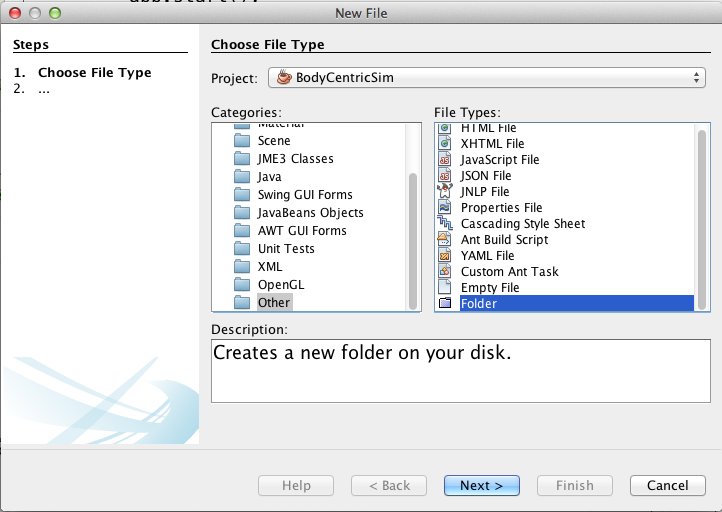
\includegraphics[width=\linewidth]{gfx/Chapter_SD_UserGuide/create_new_folder}
	\caption{Create a new folder within the Scenes folder}
	\label{fig:sd_create_folder}
\end{figure}

Copy the ''childproof.blend'' file into this folder. Once you see the file in the IDE, right click it and ''Convert to j3o Binary''. This convert it to jMonkey format.
% section sd_import_env_model (end)